% !TEX root = ../thesis.tex

\chapter{优化方案}
内存域存在的明显的嵌套关系,所以在GC过程中,当遇到多目的地问题时,必须严格按照拓扑排序迁移,整个过程是串行的。接下来我们先分析Yak GC对象迁移的算法细节,接着提出我们提高迁移并行性的优化方案。

\section{算法分析}
\subsection{追踪引用}
当epoch\_end触发时,指向存活对象的引用可能驻留在3个地方——堆、本地栈、远程栈,接下来我们从细节分析Yak是如何追踪这三种引用的。

\textbf{(1)在堆中}  \ 如果一个对象$O_b$的引用被写入另一个对象$O_a$,并且$O_a$是在另一个内存域$r^{'}$上分配的,那么$O_b$的生命期比他所在的内存域$r$更长。算法1展示了写障碍捕捉了对$O_b$的域内引用。算法1检查了一个引用是否是跨内存域/空间的引用(第2行)。如果是,被引用所属内存域(REGION($O_a$))需要更新它的记忆集(第3行)。如果$O_a$和$O_b$在相同的内存域,包括CS(第1-2行),则不需要追踪该引用。
\begin{figure}[H]
    \centering
    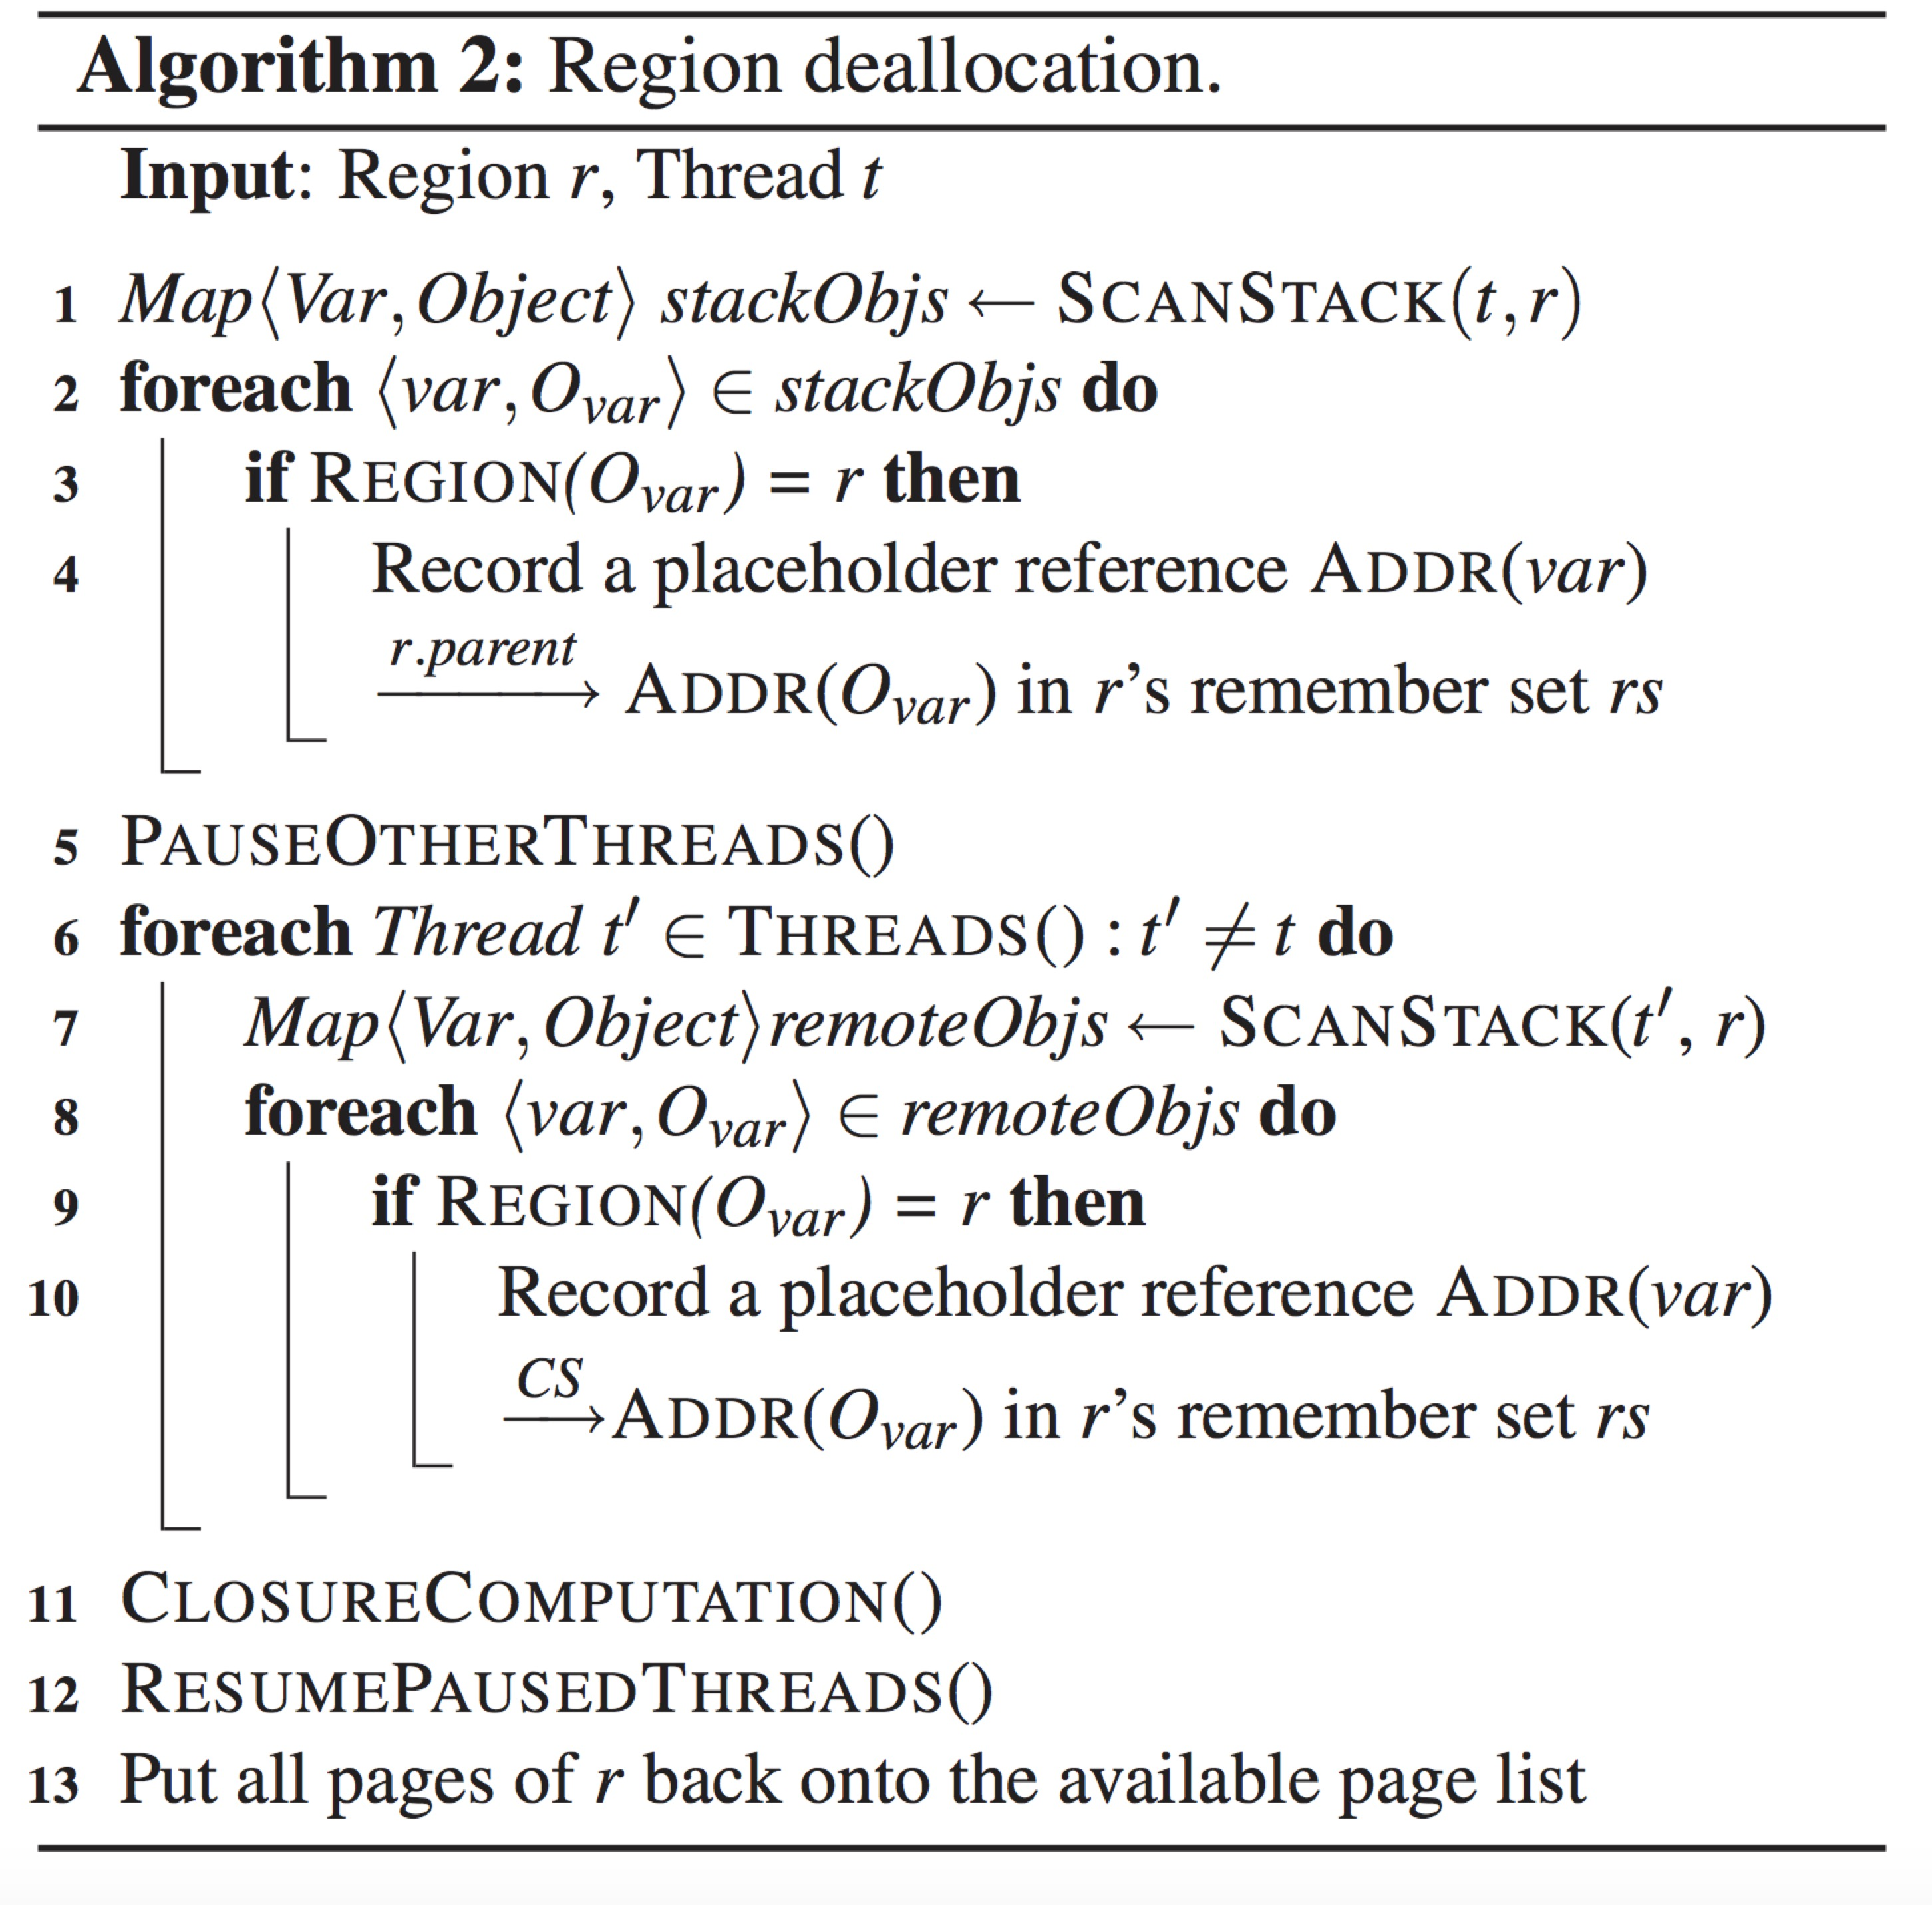
\includegraphics[width=12cm,height=12cm]{figure/algorithm2.jpg}
    \caption{
        算法2: region回收算法
    }
    \label{algorithm2}
\end{figure}

(2)\textbf{在本地栈} \ 当一个对象被运行期外的栈变量引用时,会被迁移,如图\ref{algorithm2}所示。第3行创建的对象$b$的引用被分配给栈变量$a$。$a$在$b$所属时域结束后仍活着,$b$也存活。Yak在epoch\_end后,扫描本地栈,找到$r$中所有被活引用指向的对象$O_{var}$ (算法2中1-4行),Yak在前面加上一个代表$r$的父内存域($p$)的占位符,把这条记录加入$r$的记忆集。这条记录说明着当$r$被回收,$O_{var}$ 会被迁移到$p$。

(3)\textbf{在远程栈} \ 线程$t$创建的对象$O$可能会被线程$t^{'}$中的对象引用。例如图\ref{algorithm2},第4行创建的对象,在第10行中被另一个线程$t^{'}$引用并加载到栈中。为了避免读障碍对实用性和性能的影响,Yak通过“stop-the-world”的方法保证线程的安全性。当线程$t$回收内存域$r$时,Yak暂停所有其他的线程并且扫描它们的栈。被其他线程引用的$r$内对象会被标记。

\subsection{内存域释放}
算法2展示了在每个epoch\_end触发内存域释放算法。此算法计算存活对象的闭包,将对象迁移到其目标内存域后,回收整个内存域。

\textbf{寻找转移根}:一个内存域$r$有3种转移根。第一种是$r$的记忆集中所记录的指向内存域间/空间的引用,第二种是被本地栈所引用的对象,第三种被其它线程中的远程栈所引用的对象。

由于内存域间/空间的引用早已被写障碍所捕获,Yak只要在这阶段识别出栈中引用对象。Yak首先通过的本地栈标识存活的对象,如算法2的第1-4行所示。

接下来,Yak通过远程栈标识存活的对象。为此,Yak需要将线程同步(第5行)。当远程线程暂停时,Yak扫描其栈变量,并返回一个被这些变量所引用的位于$r$中的对象的集合。每个这样的对象(远程对象)都要被明确标记为根,并在计算传递闭包之前(第11行)移动到CS(第10行)。

直到完成闭包运算并将所有的存活对象移动到它们的目标区域,没有线程会被恢复。注意,即便远程线程的栈没有引用内存域$r$中的任何对象,让其继续运行也是不安全的。

所有的存活对象都会被重新分配,然后释放整个内存域$r$,$r$占用的所有页会被重新放回空闲页表(第13行)。



算法5-1显示了从所检测到的一组转移根上计算闭包的细节。由于所有其它线程都被暂停,所以闭包计算和对象迁移是同时完成的。闭包计算是基于记忆集$rs$和当前的释放区域$r$的。首先检查了记忆集$rs$(第1行):如果$rs$为空,则该内存域不包含迁移对象,因此可以被安全地释放。否则,需标识所有的可达对象并重定位。

Yak先检查记忆集中的每个引用${addr}$  $O_{b}$的有效性,再基于半格运算计算出每个转移根$O_{b}$要移动到的目标内存域(第2-4行),这些结果保存在map $promote$中。

然后,按照所有转移根的目标区域的拓扑顺序来遍历这些转移根(第5行的循环)。对于每个转移根$O_b$,在当前区域内执行宽度优先遍历,以识别$O_b$可访问的转移对象的传递闭包,将其放入队列$gray$中。在遍历中(第8-23行),计算每个(传递)转移对象的目标内存域并移动它们。

\begin{algorithm}[H]

    
    \nonumber
    \caption{Closure computation.}%Algorithm 3:Closure computation.
    \LinesNumbered %要求显示行号
    \KwIn{Remember Set $rs$ of Region $r$}%输入参数
    %\KwOut{output result}%输出
   % some description\; %\;用于换行

    \If{The remember set $rs$ of $r$ is NOT empty}{\Delta
      \ForEach{ Escaping root $O_b$  $\in$ $rs$ }{
      \ForEach{Reference addr $\xrightarrow{r'}$ ADDR($O_b$) in rs}{
      promote[$O_b$] ← JOIN (r′, promote[$O_b$])
    }
    }
    
    \ForEach{Escaping root $O_b$ in topological order of promote[$O_b$]}{
      
    Region tgt ← promote[$O_b$]
    
    Initialize queue gray with {Ob}
    
    \While{gray is NOT empty}{
    
    Object $O$ ← DEQUEUE($gray$)
    
    Write $tgt$ into the region field of $O$
    
    Object $O^∗$ ←MOVE($O$, $tgt$)
    
    Put a forward reference at ADDR($O$)
    
    \ForEach{Reference addr $\xrightarrow{x}$ ADDR(O) in r’s rs}{
    
    Write ADDR($O^∗$) into $addr$
    
    
      \If{$x \not= tgt$}{
    
        Add reference $addr$ $\xrightarrow{x}$ ADDR($O^∗$) into the remember set of region $tgt$
    
      }
    }
    
    \ForEach{Outgoing reference e of $O^∗$}{
      
    Object O′ ← TARGET($e$)
    
    \If{$O′$ is a forward reference}{
    
    Write the new address into $O^∗$
    
    }
    
    Region r′ ← REGION(O′)
    
    \uIf { $r′ = r$ } {
    
    ENQUEUE(O′, gray);
    
    } \ElseIf {$r′\not= tgt$}
    {
    Add reference ADDR($O$) $\xrightarrow{tgt}$ADDR($O′$) into the remember set of region $r′$
    
    }
    
    
    }
    
    }
    
    
    }
    
      }
    \nonumber
    \label{a31}
    \end{algorithm}

\subsection{更新记忆集并移动对象}

因为已经暂停了所有线程,对象的移动是安全的(第11行)。当对象$O$被移动了,需要更新存储了对它的引用的所有位置(栈和堆)。可能会有3种位置:(1)内存域内位置(即来自$r$中另一个对象的引用),(2)其它内存域或 CS,(3)栈。

\textbf{(1)内存域内位置}\ 为了处理内存域内引用,遵循 GC标准,在$O$的原始位置放置一个特殊前向引用(第12行)。这将对区域内作出通知:传入的引用的位置改变了——当$O$的位置被其它引用访问时,该前向引用会被用来更新O的引用源。

\textbf{(2)来自其它区域的对象}\ 对这些对象的引用必须被记录在$r$的记忆集中。因此,可以在记忆集中发现所有对$O$的内存域间引用,并用新地址$O^{'}$更新每个这样的引用源(第14行)。由于$O^{*}$属于新内存域$tgt$,最初进入内存域$r$的引用现在会进入内存域$tgt$内。如果包含这样引用的内存域不是$tgt$,则该引用需被明确添加到${tgt}$的记忆集合中(第16行)。

将$O$移动到内存域${tgt}$也许会导致新的内存域间/空间引用(第24-25行)。比如,如果对象$O^{*}$的目标域$r^{'}$不是$tgt$ (即$O^{'}$已经被其它转移根访问过了),需要在$r^{'}$的记忆集中添加新的条目 ${ADDR}$ $\xrightarrow{x}$ $O^{*}$。


\begin{figure}[H]
    \centering
    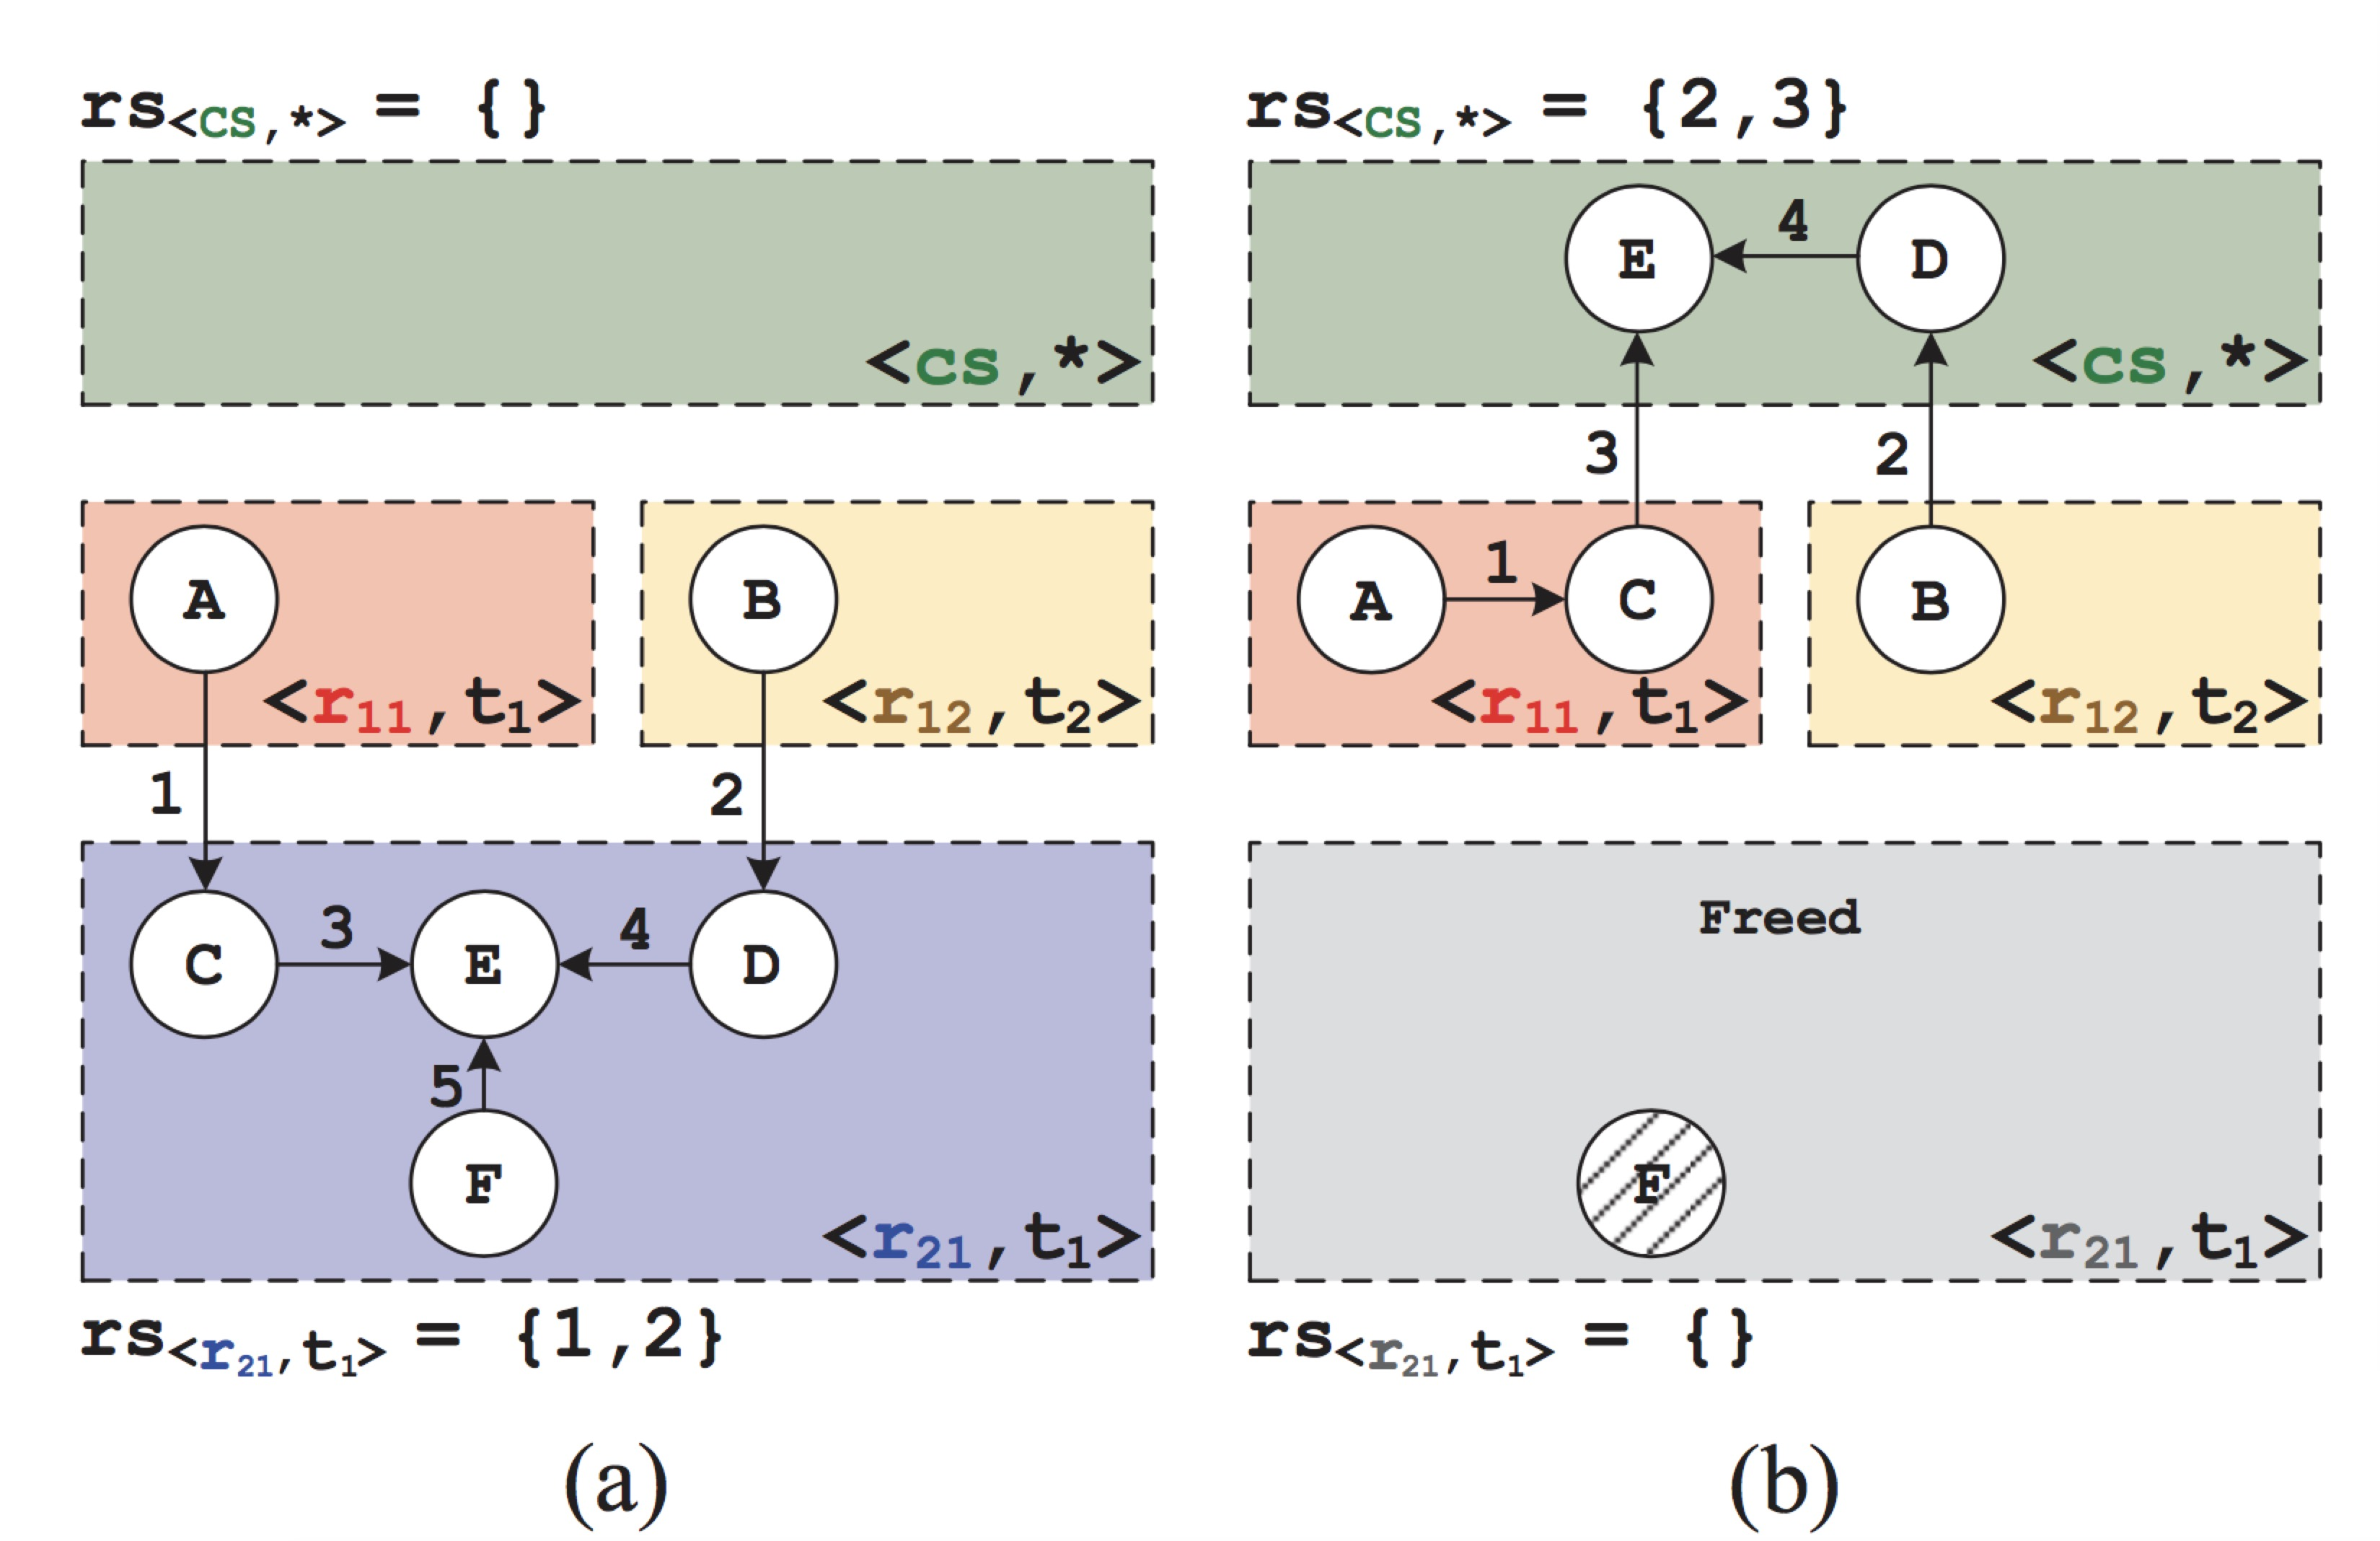
\includegraphics[width=12cm,height=7cm]{figure/snapshot.jpg}
    \caption{
        一个堆快照的例子:(a)是存活对象迁移前,(b)是迁移后。
    }
    \label{snapshot}
\end{figure}
\textbf{(3) 栈}\ 由于栈位置也被记录到记忆集中,对它们的更新方式与堆位置相同。例如,当$O$被移动了,第14行会在记忆集中更新每个对$O$的引用。如果$O$有栈引用(本地或远程),必须同样在记忆集中更新。

在传递闭包被计算和对象被迁移后,区域$r$的记忆集$rs$也就明确了(第26行)。图\ref{snapshot}显示了区域<$r_{21}$,$t_1$>被释放后的堆。对象 C、D和E是存活对象,将被移动到被计算好的目标内存域。由于D和E属于CS,在CS的记录集中添加了它们的传递引用2和3。对象F不可达,因此被自动释放。

以上就是Yak进行GC详细过程。我们注意到,在GC过程中stop-the-world是不可避免的。一是在寻找根对象时,扫描远程堆,通过stop-the-world保证线程安全,避免“危险对象移动”和“晃动对象”问题。二是在迁移对象时,避免了在其他线程正在访问将迁移对象的传递闭包,导致不完全闭包问题和当其他行程运行时,并发地移动对象,引起数据竞争问题。

stop-the-world意味着从应用中停下来并进入到GC执行过程中去。一旦stop-the-world发生,除了GC所需的线程外,其他线程都将停止工作,中断了的线程直到GC任务结束才继续它们的任务。GC调优通常就是为了改善stop-the-world的时间,我们希望能通过实现迁移对象这个过程的并行,降低迁移对象的时间,可以降低stop-the-world的时间,从而提高整个系统的性能。


\section{优化方案}

我们回到刚才的例子,Yak没有实现并行的原因就是在遇到多目的地问题时,必须严格按照拓扑排序先迁移f再迁移d,所以整个迁移过程必须是串行的。
\begin{figure}[H]
    \centering
    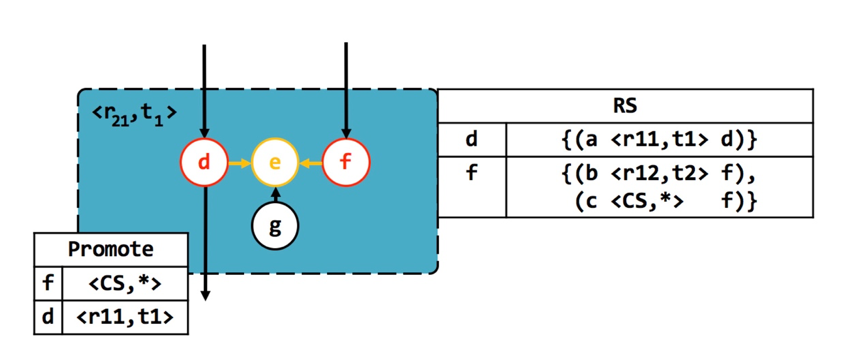
\includegraphics[width=12cm,height=5cm]{figure/n1.png}
    \caption{
        一个的多目的地迁移例子:e同时被d和f的引用,e应该迁移到层次更高的CS(f的迁移目的地)。
    }
    \label{snapshot}
\end{figure}
改进的思路是,我们可以在迁移前先进行完整的可达性分析,对含有相同对象的可达路径进行聚类,形成多个GC Task。Task内部可能存在多目的地问题,因此仍旧需要按照拓扑排序串行执行;而两个Task之间不存在交集,因此可以并行地执行对象迁移和引用更新,这样就可以提供一定的并行,进一步优化GC性能。如图\ref{snapshot},d,f,e为一个GC task;x,y,z为一个GC task;k,I,j,hl为一个GCtask。

\begin{figure}[H]
    \centering
    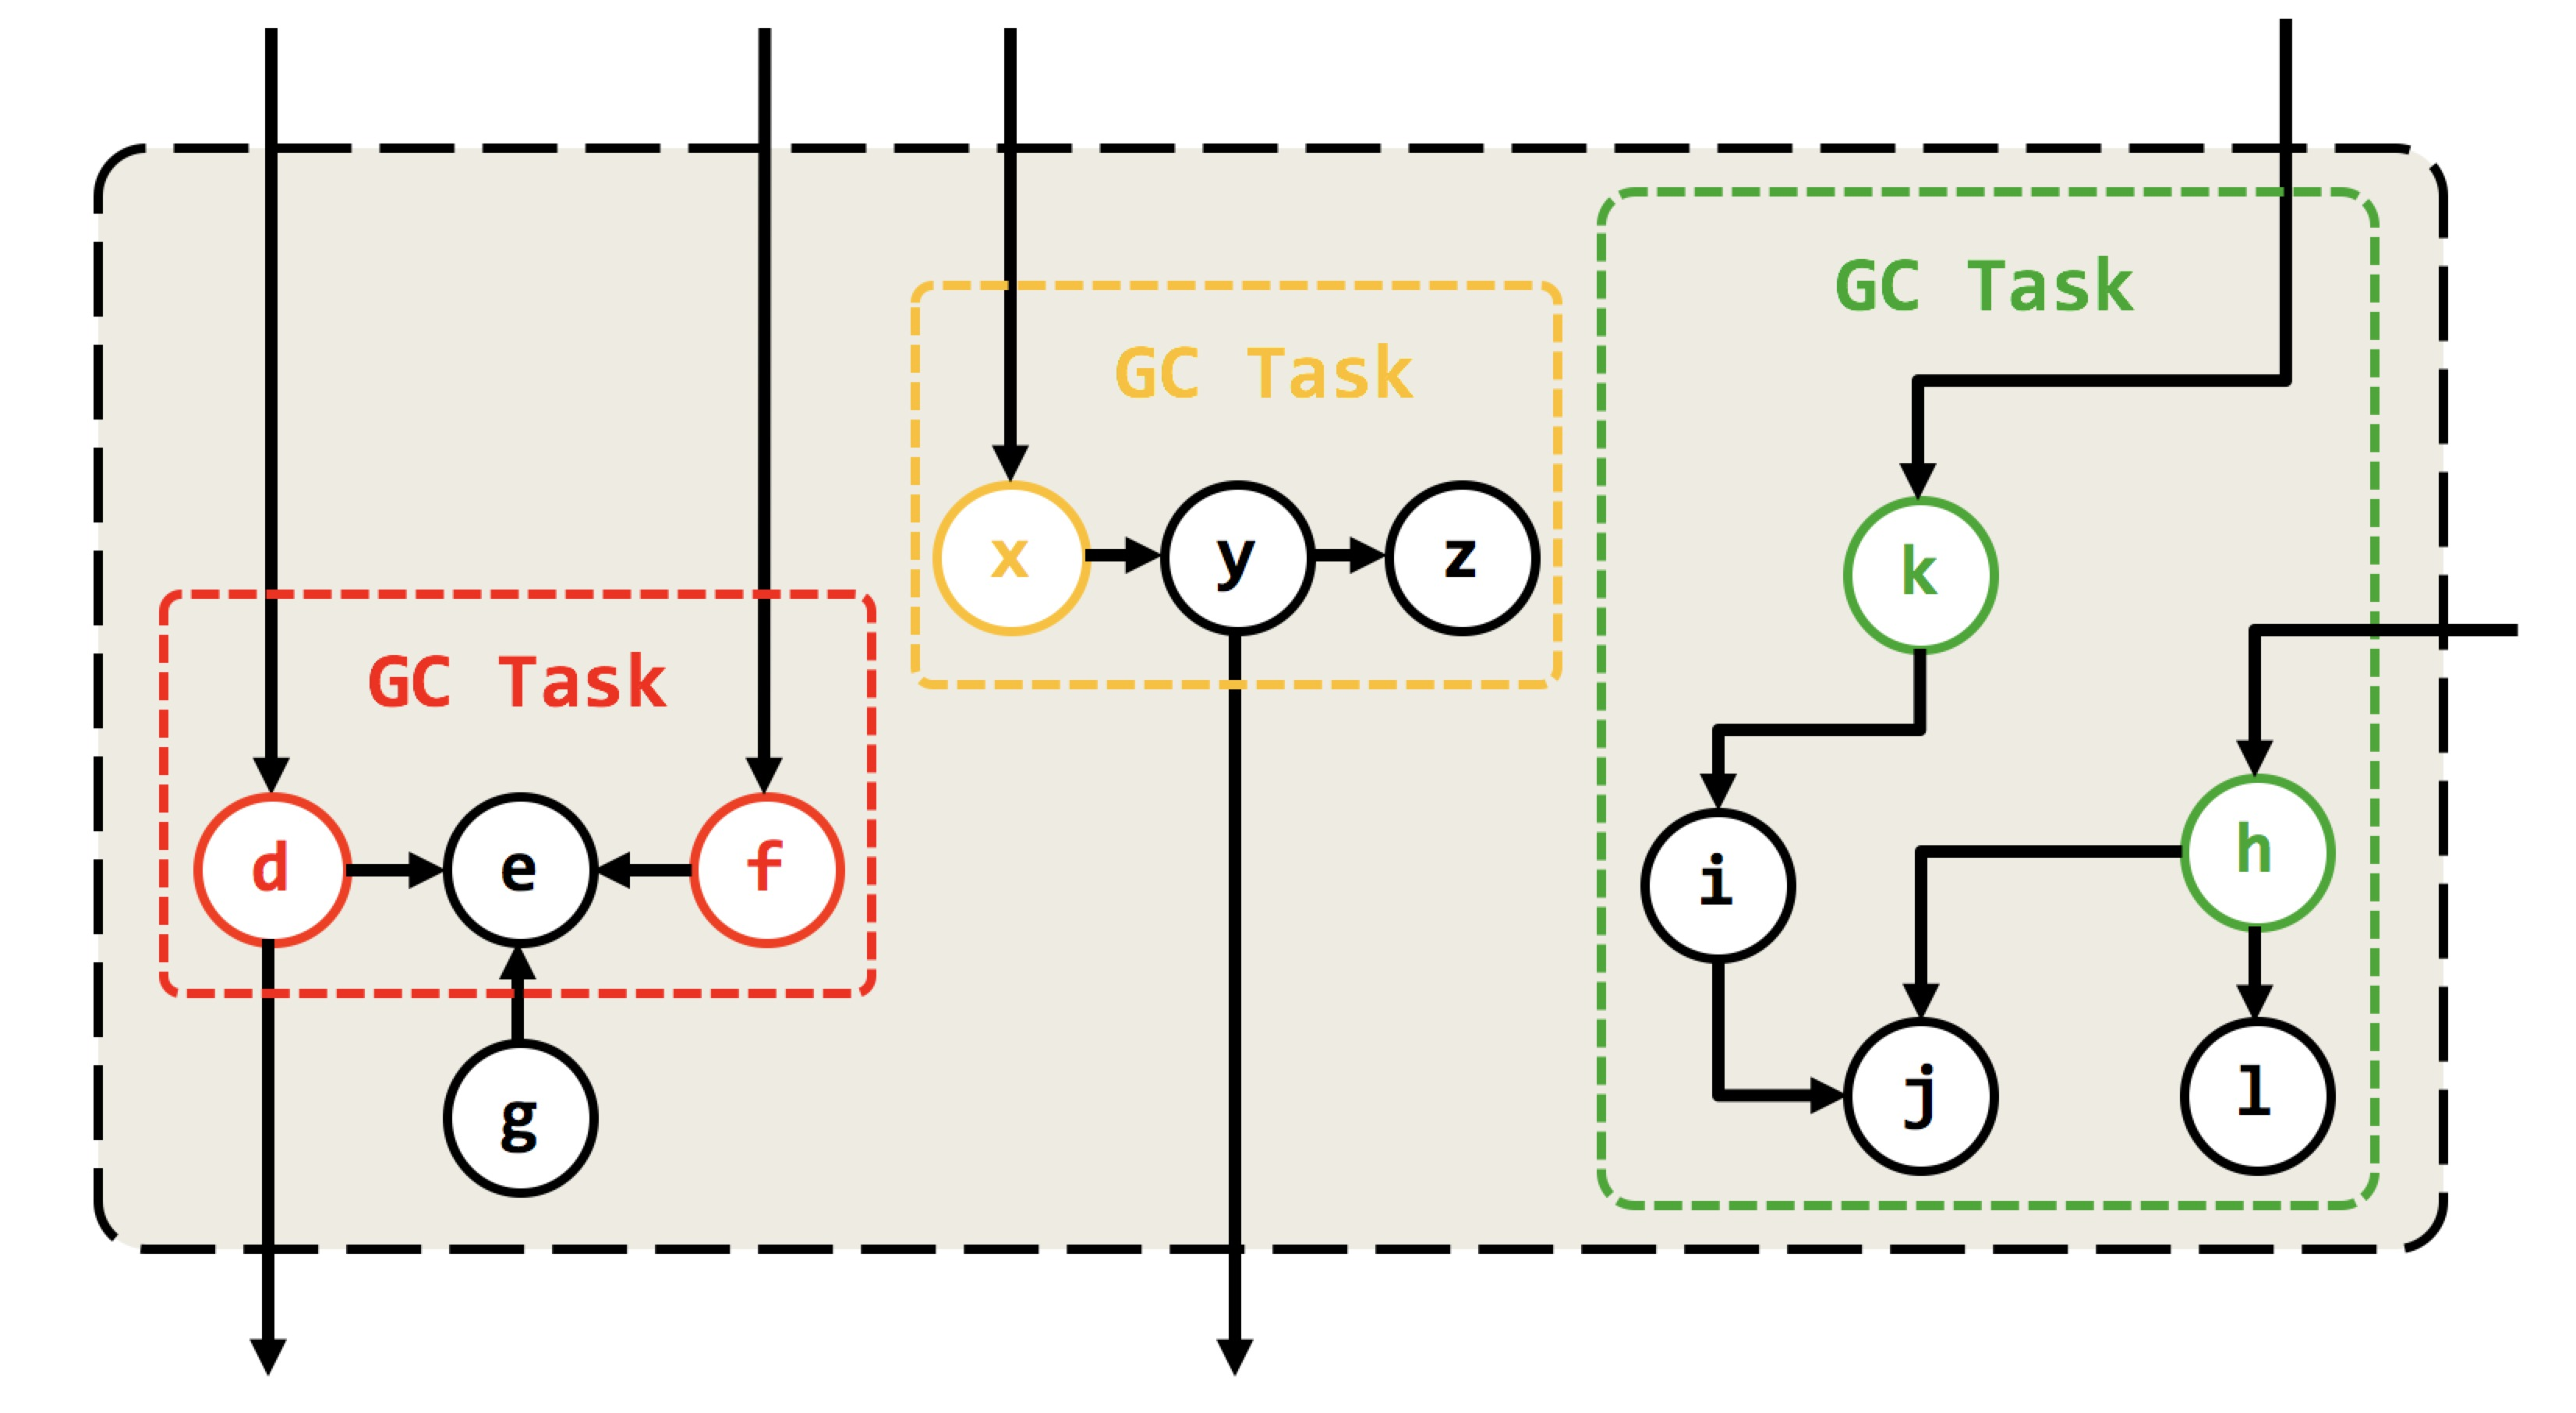
\includegraphics[width=12cm,height=7cm]{figure/n2.jpeg}
    \caption{
        GC tasks
    }
    \label{snapshot}
\end{figure}



\begin{algorithm}
    \caption{Closure computation.}%Algorithm 3:Closure computation.
    %\LinesNumbered %要求显示行号
    \KwIn{Remember Set $rs$ of Region $r$}%输入参数
    %\KwOut{output result}%输出
    % some description\; %\;用于换行
   % \begin{algorithmic}
    
    \If{The remember set $rs$ of $r$ is NOT empty}{\Delta
      \ForEach{ Escaping root $O_b$ $\in$ $rs$ }{
      \ForEach{Reference addr $\xrightarrow{r'}$ ADDR($O_b$) in rs}{
      promote[$O_b$] ← JOIN (r′, promote[$O_b$])
    }
    }
    
    Initialize map<int,set> tasks
    
    \ForEach{Escaping root $O_b$ in promote[$O_b$]}{
      
    Region tgt ← promote[$O_b$]
    Initialize queue gray with {Ob}
    
    Initialize task t\_new with {Ob}
    \While{gray is NOT empty}{
    Object $O$ ← DEQUEUE($gray$)
    
    t\_new.add(O)
    
    bool isTaskIncluded=false
    
    \ForEach{task t in tasks}{
    
    \If{t.contain(O)}{
    
    JOIN(t,t\_new)
    
    t\_new =t
    
    isTaskIncluded=true
    
    break
    }
    }
    \If{!isTaskIncluded}{
    tasks[GET\_NEW\_TASK\_ID()]=new\_t
    }
    }
    }
    
    
    
    
    
    
    
    
    
    \ForEach{task t in tasks}{
    \ForEach{Escaping root $O_b$ in topological order of task t}{
      
    Region tgt ← promote[$O_b$]
    Initialize queue gray with {Ob}
    \While{gray is NOT empty}{
    Object $O$ ← DEQUEUE($gray$)
    Write $tgt$ into the region field of $O$
    Object $O^∗$ ←MOVE($O$, $tgt$)
    Put a forward reference at ADDR($O$)
    \ForEach{Reference addr $\xrightarrow{x}$ ADDR(O) in r’s rs}{
    Write ADDR($O^∗$) into $addr$
      \If{$x \not= tgt$}{
        Add reference $addr$ $\xrightarrow{x}$ ADDR($O^∗$) into the remember set of region $tgt$
      }
    }
    
    
    
    \ForEach{Outgoing reference e of $O^∗$}{
      
    Object O′ ← TARGET($e$)
    \If{O′ is a forward reference}{
    Write the new address into $O^∗$
    }
    Region r′ ← REGION(O′)
    \uIf { r′ = r } {
    ENQUEUE(O′, gray);
    } \ElseIf {$r′\not= tgt$}
    {
    Add reference ADDR($O$) $\xrightarrow{tgt}$ADDR($O′$) into the remember set of region $r′$
    }
    }
    }
    }
    
    }
    }
    
    %\end{algorithmic}
    \end{algorithm}
   

改进的算法在5-2,1-4行依然是基于半格运算计算出每个转移根$O_b$要移动到的目标内存域,把这些结果保存在map $promote$中。第5行初始化一个map<int,set> $tasks$,用来存储分配在不同task的对象,6-19行对含有相同对象的可达路径进行聚类,放入一个task中。task拥有唯一的taskID标识,最终所有可达对象唯一存储在所属于task中。tasks存储所有task对象。

20-32行是算法并行性的实现。因为两个Task之间不存在交集,所以对每个task $t$,都有单独线程负责执行。这样通过实现迁移对象这个过程的并行,降低迁移对象的时间,可以降低stop-the-world的时间,从而提高整个系统的性能。



